\chapter{Detail design}\label{ch:detail_design}
%**********************************************
\section{Current sensor}\label{sec:current_sensor_design}
Currently being rewritten.
\subsection{Opamp configuration}\label{sec:config}


\subsection{Opamp design}
\begin{figure}
\centering
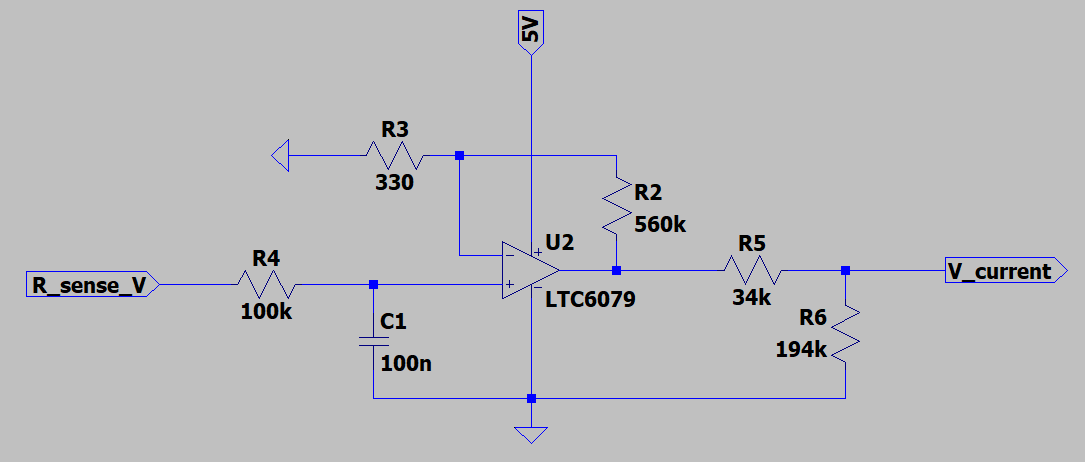
\includegraphics[width=0.65\linewidth]{./Figures/CurSens_SimCir.png}
\caption{Current sensing circuit design}
\label{fig:cursen_sim_cir}
\end{figure}

\newpage
\section{Analogue range sensor}
The HC-SR04 ultrasonic sensor requires a \SI{5}{\volt} supply and requires \SI{15}{\milli\ampere} to operate \cite{Design_SonicSens}. The frequency of the sensor output is the same as the input trigger frequency which is \SI{16}{\hertz}. Using a maximum distance of \SI{1}{\meter} and a minimum distance of \SI{5}{\centi\meter} results in a minimum duty cycle of 0.4\% and a maximum duty cycle of 10\%. The output pulses will have a maximum amplitude of  \cite{Design_SonicSens}.

Equation \ref{eqn:sens_gain} is used to calculate the needed gain of the system. In order to have the gain stage output a maximum of \SI{5}{\volt} at \SI{1}{\meter} a gain of 10.77 is required.

\begin{align}
Gain &= \frac{V_{Expected}}{V_{Duty Cycle \cdot V_{Amplitude}}}\label{eqn:sens_gain}
\end{align}

In order to determine the corner frequency fist the minimum attenuation must be calculated. The minimum attenuation can be calculated using the gain and amplitude of the first harmonic frequency component in the square wave to determine the size of the output ripple voltage, see Equation \ref{eqn:sens_harm}. Since the second harmonic and higher will all be attenuated more aggressively than the first harmonic it will contribute the most to the ripple voltage. 

\begin{align}
First Harmonic Amplitude &= V_{Amplitude} \cdot DutyCycle \cdot sinc(\pi \cdot DutyCycle)\label{eqn:sens_harm}\\
MinimumAttenuation &= 20log(\frac{MaximumNoise}{FirstHarmonicAmplitude \cdot Gain})\label{eqn:sens_atten}
\end{align}

Using Equation \ref{eqn:sens_atten} it is determined that an attenuation of atleast \SI{-41}{\decibel} is needed at \SI{16}{\hertz}. The corner frequency is then determined solving a simple straight line graph equation as shown in Equation \ref{eqn:sens_cutoff}.

\begin{align}
log(w) &= \frac{MinimumAttenuation+AttenuationSlope \cdot log(2\pi \cdot F_{trigger})}{AttenuationSlope}\\
F_{cutoff} &= 10^{2\pi \cdot log(w)}\label{eqn:sens_cutoff}
\end{align}

To determine what order filter to use Equation \ref{eqn:sens_cutoff} was solved using the different gradients for 1st, 2nd and 3rd order filters. Table \ref{tbl:sens_cutoff} shows the results of these calculations. In order to adhere to the response time specifications of \SI{1.5}{\second} it was decided that a 3rd order filter would have the best response time and noise attenuation without being to complex to build. 

\begin{table}\label{tbl:sens_cutoff}
\begin{center}
\begin{tabular}{|c|c|c|}
\hline
Filter & Gradient & Maximum corner frequency\\
\hline
1st & \SI{-20}{\decibel} & \SI{0.13}{\hertz}\\
2nd & \SI{-40}{\decibel} & \SI{1.44}{\hertz}\\
3rd & \SI{-60}{\decibel} & \SI{3.2}{\hertz}\\
\hline
\end{tabular}
\end{center}
\caption{Filters and their maximum required corner frequency}
\end{table}

Design document \cite{Design_SonicSens_Filter} was used in the design of the 3rd order filter. Figure: \ref{fig:sonicsens_filter} shows the filter configuration that will be used. A simple gain stage will be appended to the end of the filter and then a voltage divider will ensure that the final output voltage is less than \SI{3.3}{\volt}. The whole circuit diagram is shown in Figure: \ref{fig:sonicsens_diag}. The circuit is designed to take input with an amplitude of \SI{5}{\volt} with a duty cycle between 0\% and 10\%.

The design document gives nominal values of R1=\SI{1.6}{\kilo\ohm} R2=\SI{2.4}{\kilo\ohm}  R3=\SI{7.5}{\kilo\ohm} C1=\SI{100}{\nano\farad} C2=\SI{10}{\nano\farad} C3=\SI{47}{\nano\farad} to construct a third order filter with a  corner frequency of \SI{1}{\kilo\hertz}. It was decided to design for a corner frequency of \SI{2}{\hertz} as this provides a good compromise between noise reduction and response time. In order to achieve this corner frequency frequency and impedance scaling was used on the given component values to get them to acceptable values that are easy to implement and result in minimal current draw. 


For the gain stage resistors R5 = \SI{22}{\kilo\ohm} and R6 = \SI{220}{\kilo\ohm} potentiometer. This will allow for a gain of up to 10 as calculated, however as shown in Figure: \ref{fig:sonicsens_diag} a lower gain is required to achieve the desired circuit response. This is due to practicalities such as rise time increasing the DC component of the input signal.


The voltage divider, R7 and R8 in Figure: \ref{fig:sonicsens_diag}, is to reduce the maximum output of \SI{5}{\volt} from the gain stage to a maximum of \SI{3.3}{\volt} to be used as input to the micro-controller. The resistor values are chosen to reduce current draw.

\begin{figure}
\centering
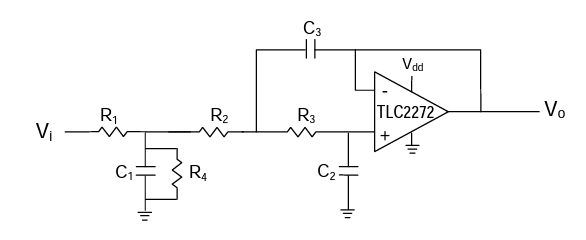
\includegraphics[width=0.5\textwidth]{./Figures/SonicSens_Filter.png}
\caption{Filter configuration from \cite{Design_SonicSens_Filter}}
\label{fig:sonicsens_filter}
\end{figure}

\begin{figure}
\centering
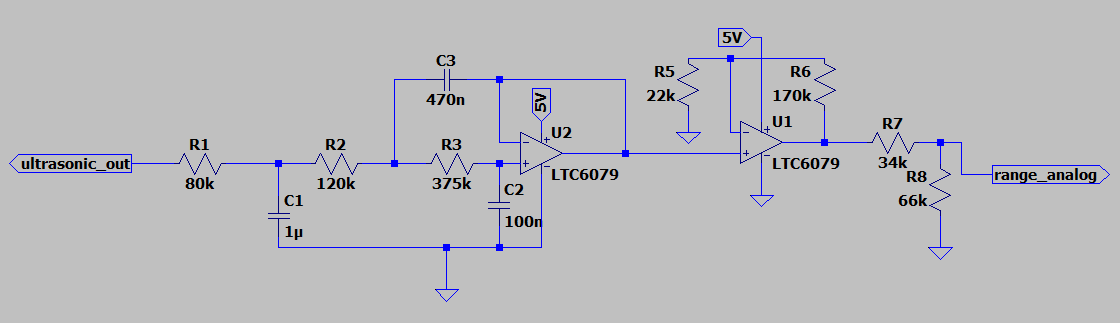
\includegraphics[width=0.5\textwidth]{./Figures/SonicSens_Diagram.png}
\caption{Filter configuration from \cite{Design_SonicSens_Filter}}
\label{fig:sonicsens_diag}
\end{figure}







